\documentclass[12pt,border=0pt]{standalone}

\usepackage[utf8]{inputenc} 
\usepackage{amssymb,amsmath}
\usepackage{tikz}
\usetikzlibrary{positioning, arrows} 


\thispagestyle{empty}

\begin{document}

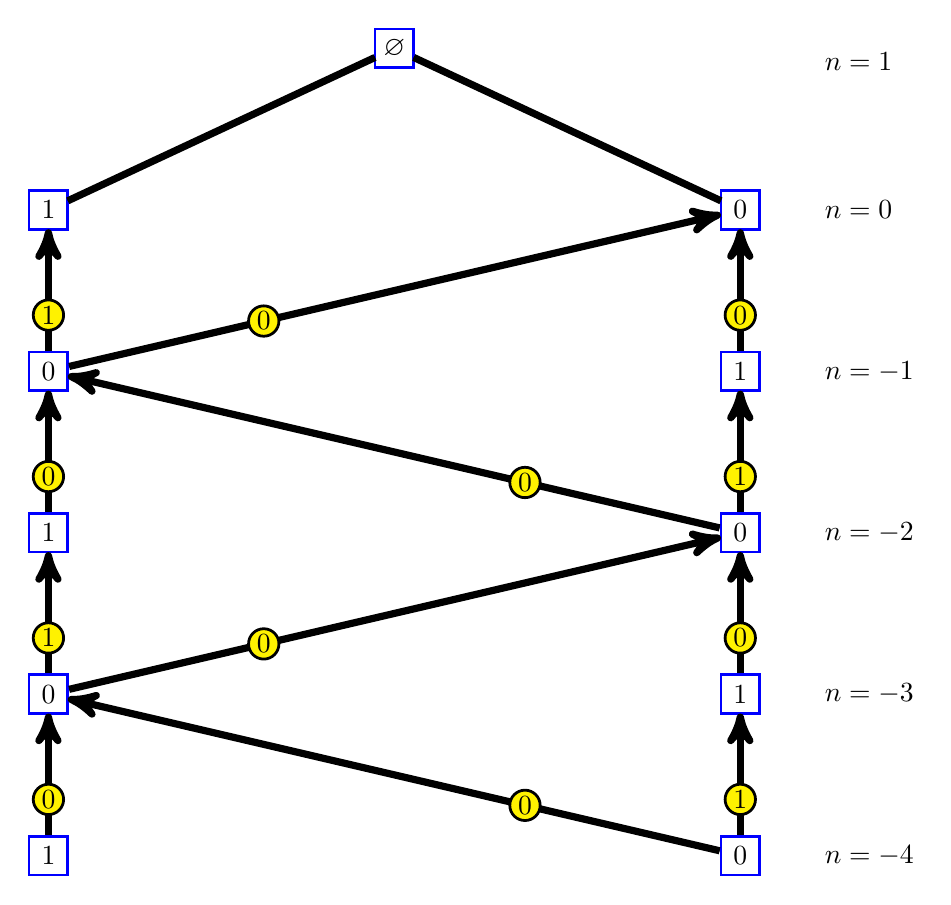
\begin{tikzpicture}[x=10pt,y=7pt]
  \centering
  \tikzset{VertexStyle/.style = {
    shape         = rectangle,
    draw          = blue, 
    fill          = white, 
  	line width    = 1pt, 
    text          = black,
    inner sep     = 1pt,
    outer sep     = 0pt,
    minimum size  = 14 pt,
    scale         = 1
    }
  }
  \tikzset{EdgeStyle/.style = {
    draw            = black, 
    thick,
    double          = black,
    double distance = 1pt,
    <-,>=stealth',shorten >=0.5pt
    }
  }
  \tikzset{EdgeEmpty/.style = {
    draw            = black, 
    thick,
    double          = black,
    double distance = 1pt
    }
  }
  \tikzset{EdgeLabelStyle/.style = {
    draw          = black,
  	shape         = circle, 
  	line width    = 1pt, 
  	minimum size  = 10pt, 
    inner sep     = 1pt,
    outer sep     = 0pt,
    fill          = yellow,
    text          = black,
    scale         = 1,
    pos=0.7
    }
  }

	\node[VertexStyle](A1) at (25, 45.8333333333333) {$\varnothing$};
	\node[VertexStyle](B1) at (12.5, 37.5) {$1$};
	\node[VertexStyle](B2) at (37.5, 37.5) {$0$};
	\node[VertexStyle](C1) at (12.5, 29.1666666666667) {$0$};
	\node[VertexStyle](C2) at (37.5, 29.1666666666667) {$1$};
	\node[VertexStyle](D1) at (12.5, 20.8333333333333) {$1$};
	\node[VertexStyle](D2) at (37.5, 20.8333333333333) {$0$};
	\node[VertexStyle](E1) at (12.5, 12.5) {$0$};
	\node[VertexStyle](E2) at (37.5, 12.5) {$1$};
	\node[VertexStyle](F1) at (12.5, 4.16666666666667) {$1$};
	\node[VertexStyle](F2) at (37.5, 4.16666666666667) {$0$};
	\draw[EdgeEmpty](A1) to (B1);
	\draw[EdgeEmpty](A1) to (B2);
	\draw[EdgeStyle](B1) to node[EdgeLabelStyle]{$1$} (C1);
	\draw[EdgeStyle](B2) to node[EdgeLabelStyle]{$0$} (C1);
	\draw[EdgeStyle](B2) to node[EdgeLabelStyle]{$0$} (C2);
	\draw[EdgeStyle](C1) to node[EdgeLabelStyle]{$0$} (D1);
	\draw[EdgeStyle](C1) to node[EdgeLabelStyle]{$0$} (D2);
	\draw[EdgeStyle](C2) to node[EdgeLabelStyle]{$1$} (D2);
	\draw[EdgeStyle](D1) to node[EdgeLabelStyle]{$1$} (E1);
	\draw[EdgeStyle](D2) to node[EdgeLabelStyle]{$0$} (E1);
	\draw[EdgeStyle](D2) to node[EdgeLabelStyle]{$0$} (E2);
	\draw[EdgeStyle](E1) to node[EdgeLabelStyle]{$0$} (F1);
	\draw[EdgeStyle](E1) to node[EdgeLabelStyle]{$0$} (F2);
	\draw[EdgeStyle](E2) to node[EdgeLabelStyle]{$1$} (F2);

	\node[right=20pt of B2](n0) {$n=0$};
	\node[above=40pt of n0] {$n=1$};
	\node[right=20pt of C2] {$n=-1$};
	\node[right=20pt of D2] {$n=-2$};
	\node[right=20pt of E2] {$n=-3$};
	\node[right=20pt of F2] {$n=-4$};
	
  \end{tikzpicture}

\end{document}
